\section{Example 1 - Infinite Bus}
In this section, we assess how the proposed methods can be applied to study the stability of a converter connected to the infinite bus system described earlier. Moreover, we address the conservativeness limitation showed in Section \ref{sec:lim} and how this can be resolved with a proper choice of the weighting matrix $W_i(s)$.

\subsection{Virtual Admittance compensation}
Figure \ref{fig:GFM_gain_phase_test} shows that, even when both systems are sectorial, the small-phase eigenvalue bounds are highly conservative for frequencies below $50$ Hz. This conservatism arises from the fact that both of $Y_C$ and $Y^{-1}_{net}$ exhibit large phases, and, recalling \eqref{eq:phase_bound}, the small-phase bound is derived under a worst-case assumption, pairing maxima with maxima and minima with minima. However, favorable phase interactions may occur in the product $Y_CY^{-1}_{net}$, leading to partial compensation and a reduction of its eigenvalues' phase. This phenomenon is evident in Figure~\ref{fig:phase-bounds_Yv}, where the small-phase bounds $\Phi(Y_C)+\Phi(Y_{net}^{-1})$ clearly overestimate the actual eigenvalues' phase $\angle\lambda(Y_CY_{net}^{-1})$.

A tighter bound can be obtained by reducing the large phase spread of the numerical range, and therefore limiting the extreme combinations of phases. Since the converter implements a virtual admittance control $Y_v(s)$, and its behavior around $50$ Hz is mainly determined by the virtual admittance, we can post-multiply $Y_C(s)$ by the inverse of $Y_{v}(s)$, such that $Y_{C}(s)Y_{v}(s)^{-1}\approx I$ around those frequencies. The network admittance is transformed accordingly to $Y_{net}(s)Y_{v}(s)^{-1}$.
%we select the post-multiplication matrix $\mathcal{F}(s)=Y_{virt}(s)^{-1}$ (with $\mathcal{E}=I$, $\mathcal{C}=0$). So that we obtain $\tilde{J}_c(s)\approx I$. Meanwhile, $\tilde{J}_{net}(s)= Y_{net}(s)Y_{virt}(s)^{-1}$. 
From another viewpoint, a known dynamic behaviour is shifted from the converter to the network, thereby avoiding the conservatism.
Figure~\ref{fig:phase-bounds_Yv} illustrates the effect of this compensation. It can be seen that applying the proposed virtual admittance filtering leads to noticeably improved bounds.
This figure also highlights the necessity of the translation term $\mathcal{C}$. Since one eigenvalue’s phase approaches $\pi$ at low frequencies and pre-/post-multiplication does not alter it, we must rely on the small gain at those frequencies to ensure stability. Conversely, with a properly chosen $\mathcal{C}$, the stability assessment can rely solely on the phase criterion, as discussed in the next subsection.
%Notice that, since $\mathcal{E}$ and $\mathcal{F}$$ do not change the eigenvalues phase of open-loop system, and since the phase of one of the eigenvalues tends to $pi$ for frequency tending to zero, then we cannot guarantee stability by just

At first glance, this approach may appear to undermine the decentralized nature of the certificate. However, in practice, exact knowledge of the virtual admittance values (that is, the behaviour around $50$Hz) is not required, and approximate values are sufficient, as shown afterwards. In a decentralized setting, these values can either be selected a priori as fixed parameters or assigned differently across units by the stability certifier. In any case, proposed grid codes for grid-forming converters already define fixed ranges for the effective impedance~\cite{entsoe}. 
%In Figure~\ref{fig:phase-vi-filt}, the small-phase criteria is shown when the post-filter $Y_{virt}(s)$ is used. We can notice that, compared to Figure \ref{fig:GFM_gain_phase_test}, the phase spread of each system is reduced and the phase margin between converter and network is increased.

\begin{figure}[tb]
    \centering
    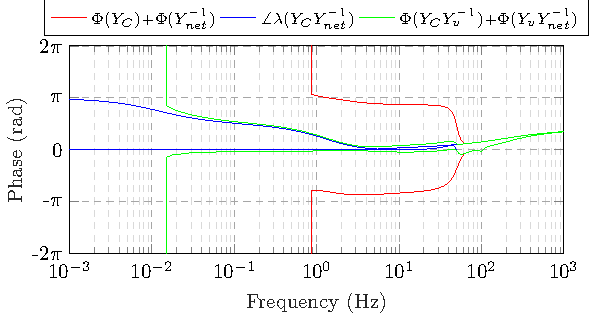
\includegraphics[width=\linewidth]{1_Phase_Bounds.pdf}
    \caption{Small-phase bounds without and with virtual admittance compensation.}
    \label{fig:phase-bounds_Yv}
    \vspace{-1em}
\end{figure}

%\begin{figure}[tbh]
%    \centering
%    \includegraphics[width=\linewidth]{Figures/GFM_InfBus_Yvirt/Phase.pdf}
%    \caption{Small phase condition of a GFM converter with virtual admittance post-filtering.}
%    \label{fig:phase-vi-filt}
%\end{figure}

\subsection{Full transformation}

In Figure~\ref{fig:phase-dep-frame} the small-phase criteria is shown with the frequency-depended transformation \eqref{eq:generic_trasnf}, which matrices are defined as in~\eqref{eq:freq_dep_tf_better}. Compared to the previous results, we can obtain sectoriality for the full frequency range and the closed-loop system stability is guaranteed by the small-phase conditions.

%This also suggests that the converter remains stable under any network short-circuit ratio, since the network impedance phase depends only on the R/X ratio, not on the impedance magnitude. This holds without power transfer, since network impedance does not affect the operating point or converter admittance. With power transfer, further analysis is needed.

\begin{figure}[t]
    \centering 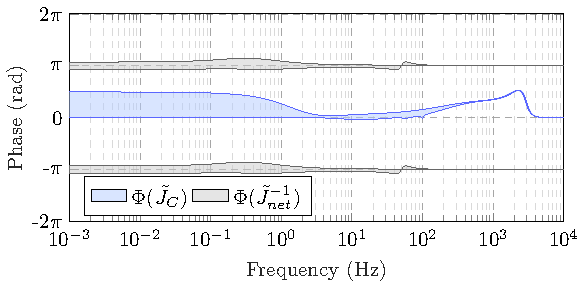
\includegraphics[width=\linewidth]{2_Phase.pdf}
    \caption{Small phase condition of a GFM converter with frequency-dependent transformation \eqref{eq:generic_trasnf}, \eqref{eq:freq_dep_tf_better}.}
    \label{fig:phase-dep-frame}
    %\vspace{-1em}
\end{figure}

\subsection{Unstable case}
To further validate the method, we examine the sufficient condition of the theorem: if the closed-loop system is unstable, then the small-phase and the small-gain condition must be simultaneously violated at some frequency. In practice, destabilizing a grid-forming converter is not straightforward. Following \cite{de2012automatic}, we introduce a purely resistive load at the PCC and increase the infinite bus impedance. By switching the control mode to constant-Q and reducing the SVM damping of the GFM from $0.5$ to $0.05$, the closed-loop becomes unstable, exhibiting sustained oscillations at 1.2 Hz. Figure \ref{fig:GFM_Unstable} illustrates the mixed gain/phase test, considering the proposed transformation. 
Enabling the reactive power control reduces the gain at low frequencies, leading to the small-gain condition to be satisfied.
However, while in the stable case ($D=0.5$) the small-phase condition is satisfied, in the unstable case ($D=0.05$), the converter phase increases substantially, and together with the network phase causes the phase condition to be violated, while the gain condition is also not satisfied around the unstable oscillation frequency.
\section{Example 2 - IEEE 14 Bus System}
\begin{figure}[t]
    \centering
    \begin{subfigure}{\columnwidth}
        \centering
        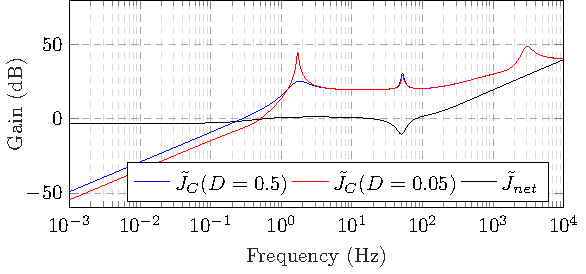
\includegraphics[width=\linewidth]{3_Gain.pdf}
    \end{subfigure}
    \begin{subfigure}{\columnwidth}
        \centering
        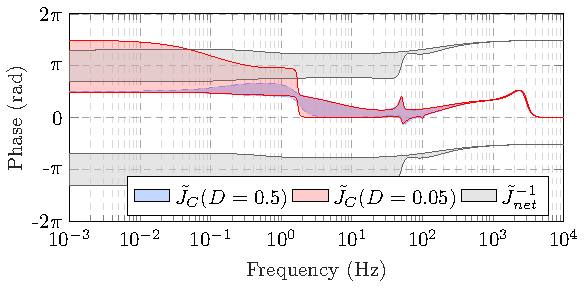
\includegraphics[width=\linewidth]{3_Phase.pdf}
    \end{subfigure}
    \caption{GFM Infinite Bus - Stable vs Unstable.}
    \label{fig:GFM_Unstable}
    \vspace{-1em}
\end{figure}
To extend and show the scalability of our approach, we consider the modified IEEE 14 Bus System \cite{Repo}. Four GFM converters are connected at the buses 2, 3, 6, and 8.
Similarly to the infinite bus example, to build an unstable case, we select a low damping value for converter 8, connect purely resistive loads, and increase the line 8-9 impedance. In this setup, the system is unstable with an unstable oscillation at 0.54 Hz.
In Figure \ref{fig:IEEE14_criteria}, the decentralized conditions are shown. While the converters 2, 3, and 6 satisfy the small-phase condition, converter 8 does not. In particular, below 1.64 Hz, its phase overlaps the network phase. This does not imply the instability of the system; however, knowing that the system is unstable, it identifies the responsible converter, and by appropriately retuning its control parameters, stability can potentially be restored. For example, if we apply the same tuning of converter 6, which satisfy the small-phase condition, to converter 8, then stability is recovered.

In this example, each converter implements a different virtual admittance value, while the same value is applied to all converters for the transformation in~\eqref{eq:freq_dep_tf_better}. This shows that, even when the exact virtual admittance is unknown, it is still possible to use a reasonable estimate to obtain adequate phase bounds and thus an effective stability validation with the proposed approach.
\begin{figure}[t]
    \centering
    \begin{subfigure}{\columnwidth}
        \centering
        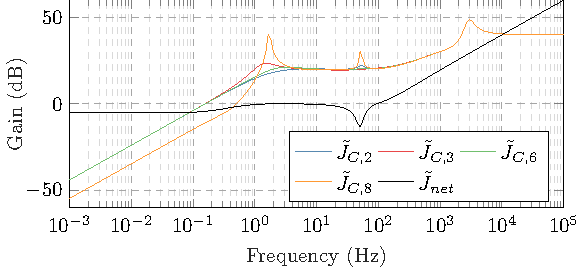
\includegraphics[width=\linewidth]{5_Gain.pdf}
    \end{subfigure}
    %\vspace{-1em} 
    \begin{subfigure}{\columnwidth}
        \centering
        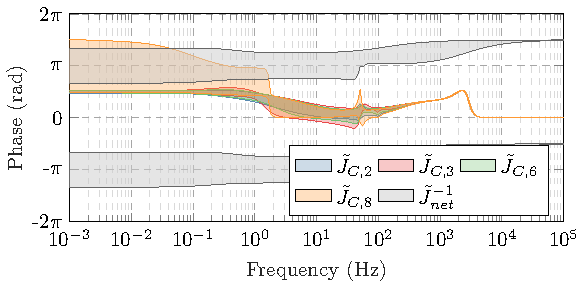
\includegraphics[width=\linewidth]{5_Phase.pdf}
    \end{subfigure}
    \caption{IEEE14 Bus system}
    \label{fig:IEEE14_criteria}
    \vspace{-1em}
\end{figure}
We intentionally excluded GFL converters. Although the concepts presented are general and applicable to different control structures, GFL converters exhibit distinct dynamics that require a separate, more detailed analysis and potentially a different definition of the transformation matrices. Furthermore, as highlighted in \cite{huangGainPhaseDecentralized2024}, the small-gain condition plays a more critical role, making it necessary to shift the high gain of GFMs toward the network to enhance its strength.